\chapter{The Mathematical Background}
\label{ch:MB}

\section{Probability theory}

Probability theory is a part of mathematics that deals with mathematical models of trials
whose outcomes depend on chance. For the perspective of mathematical finance, we will go through
some basic concepts of probability theory that are needed to begin solving stochastic calculus
problems. It is not completed the whole prospect, but be sufficient for this research. %In particular, pricing the Black-Schole-Merton model and European barrier call option with rebates.
%We consider an experiment or a trial whose outcome is not predictable with certainty.
%The set of all possible outcomes of an experiment is called the sample space and we denote it
%by $\Omega$. Any subset A of the sample space is known as an event, where an event is a set consisting
%of possible outcomes of the experiment.
%The collection of events can be defined as a subcollection $\mathcal{F}$ of the set of all subsets of $\Omega$
%and we define any collection $\mathcal{F}$ of subsets of $\Omega$. \\


\subsection{Continuous Random Variables}
A continuous random variable is a random variable where the data can take infinitely many values. For example, heights of people in a population. Let's X is a continuous random variable, the cumulative distribution $F$ of $X$ is given by
\begin{align*}
	F(x) = P\{X\leq x\}
\end{align*}
We shall assume that there is some function f such that
\begin{align*}
		F(x) = \displaystyle \int_{-\infty}^{x}f(t)dt
\end{align*}
for all real number $x$, $f$ is known as the PDF for X. The PDF $f$ of a continuous random variable X satifies
\begin{enumerate}
	\item $f(x) \geq 0$ for all $x$;
	\item $\int_{-\infty}^{\infty}f(x)dx = 1$
	\item $P(a\leq X \leq b)=\int_{a}^{b}f(x)dx$ for all $a, b$.
\end{enumerate}
\begin{figure}[htp]
	\begin{center}
		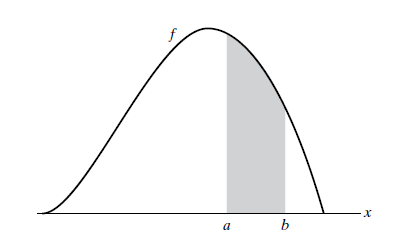
\includegraphics[scale=0.8]{figure6}
	\end{center}
	\label{reffig6}
	\caption{$P(a\leq X \leq b)$ = area of shaded region. }
\end{figure}
Probabilities correspond to areas under the curve $f(x)$. For any single value a, $P(X=a)=0$.\\
$P(a< X < b)=P(a\leq X < b)=P(a< X \leq b)=P(a\leq X \leq b)$.\\
The expected value of $X$,
\begin{align*}
	E[X] = \displaystyle \int_{-\infty}^{\infty}xf(x)dx
\end{align*}
The expected value of any real-valued function g,
\begin{center}
	$E[g(x)] = \displaystyle \int_{-\infty}^{\infty}g(x)f(x)dx$
\end{center}
The variance
\begin{align*}
	Var(X) = E[(X - \mu)^2] &= E[X^2]-(E[X])^2\\
	Var(aX+b) &= a^2\sqrt{Var(X)}
\end{align*}
Where\\
 $\mu$ : expected value of X\\
 $a, b$: real value
 
 \newpage
\subsection{Normal Random Variables}
	\begin{figure}[htp]
	\begin{center}
		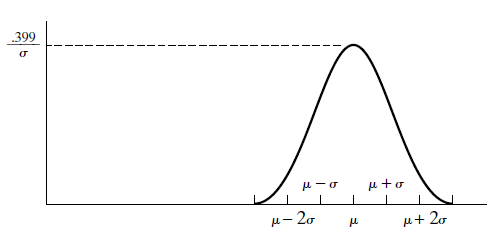
\includegraphics[scale=0.8]{figure3}
	\end{center}
	\label{reffig3}
	\caption{Arbitrary $\mu$, $\sigma^2$}
\end{figure}
X is a normal random variable (normally distributed) with parameter $\mu$ and $\sigma^2$, the density of X is given by
\begin{center}
	$f(x)=\dfrac{1}{\sqrt{2\pi}\sigma}e^\frac{-(x-\mu)^2}{2\sigma^2}  \hspace{3cm} -\infty\hspace{0.2cm}<\hspace{0.2cm} x\hspace{0.2cm}<\hspace{0.2cm}\infty$
\end{center}
If $Y=aX+b$, then $Y$ is normally distributed with parameter $a\mu+b$ and $a^2\sigma^2$.
\begin{itemize}
	\item The cumulative distribution of $Y$
	\begin{center}
		$F_Y(x)=P\{Y\leq x\}=F_X\left(\dfrac{x-b}{a}\right)$
	\end{center}
	\item The density function of $Y$
	\begin{center}
		$f_Y(x)=\dfrac{1}{\sqrt{2\pi}a\sigma}e^\frac{-(x-b-a\mu)^2}{2(a\mu)^2}$
	\end{center}
\end{itemize}

\newpage
\subsubsection*{The standard normal random variable}
	\begin{figure}[htp]
	\begin{center}
		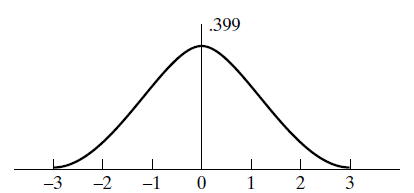
\includegraphics[scale=0.8]{figure4}
	\end{center}
	\label{reffig4}
	\caption{$\mu=0$, $\sigma=1$}
\end{figure}

$Z=\dfrac{X-\mu}{\sigma}$ is standard normally distributed with parameters $0$ and $1$.\\[0.5cm]
\indent{\itshape\bfseries Proof}\\[0.5cm]
Mean parameter
\begin{align*}
	E\left(\dfrac{X-\mu}{\sigma}\right) &=\dfrac{1}{\sigma}E(X-\mu)=\dfrac{1}{\sigma}[E(X)-E(\mu)]\\
	&=\dfrac{1}{\sigma}(\mu - \mu)=0.
\end{align*}
Volatility parameter
\begin{align*}
	Var\left(\dfrac{X-\mu}{\sigma}\right)
	&=\dfrac{1}{\sigma^2}Var(X-\mu)=\dfrac{1}{\sigma^2}[Var(X)-Var(\mu)]\\
	&=\dfrac{\sigma^2}{\sigma^2}=1.		
\end{align*}
The cumulative distribution function of standard normal random variable
\begin{align}
	\phi(x)&=\dfrac{1}{\sqrt{2\pi}} \displaystyle \int_{-\infty}^{x}e^\frac{-y^2}{2}dy \label{eq2.2.1} \\
	\phi(-x)&=1-\phi(x) \label{eq2.2.2}
\end{align}
\indent{\itshape\bfseries Proof}\\[0.5cm]
\indent Firstly, equation \eqref{eq2.2.1}\\
\indent Let $Y=\dfrac{X-\mu}{\sigma}$, then
\begin{align*}
	\phi(x)&=\displaystyle\int_{-\infty}^{x}\dfrac{1}{\sqrt{2\pi}\sigma}e^\frac{-(y-\mu)^2}{2\sigma^2}dy\\
	&=\displaystyle\int_{-\infty}^{x}\dfrac{1}{\sqrt{2\pi}\times1}e^\frac{-(y-0)^2}{2\times1^2}dy\\
	&=\dfrac{1}{\sqrt{2\pi}} \displaystyle \int_{-\infty}^{x}e^\frac{-y^2}{2}dy
\end{align*}
Secondly, equation \eqref{eq2.2.2} 
\begin{align*}
	\phi(-x)&=P\{X< -x\}\\
	&=P\{X> x\}\\
	&=P\{X\in (x,\infty)\}\\
	&=\dfrac{1}{\sqrt{2\pi}} \displaystyle \int_{x}^{\infty}e^\frac{-x^2}{2}dx\\
	&=\dfrac{1}{\sqrt{2\pi}} \displaystyle \int_{-\infty}^{\infty}e^\frac{-x^2}{2}dx - \dfrac{1}{\sqrt{2\pi}} \displaystyle \int_{-\infty}^{x}e^\frac{-x^2}{2}dx\\
	&=1 - \phi(x)
\end{align*}

\subsection{Lognormal property of stock price}
We have a random variable Y
\begin{center}
	$Y=e^X\sim$ $\log-N(\mu, \sigma^2)$ is distributed log-normally,\\ [0.3cm]
	then $\ln Y=X\sim N(\mu, \sigma^2)$ is normally distributed
\end{center}
The lognormal distribution is bounded below by $0$ and skewed to the right. It is extremely useful when analyzing stock prices which cannot fall below zero.
\begin{figure}[htp]
	\begin{center}
		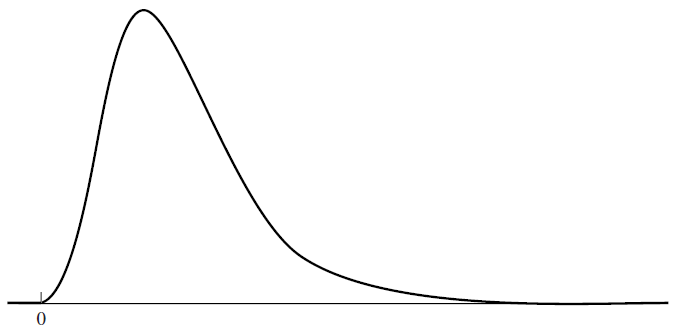
\includegraphics[scale=0.5]{figure7}
	\end{center}
	\label{reffig7}
	\caption{Lognormal distribution}
\end{figure}\\

\newpage
The mean value and variance of the log-normal distribution is given by
\begin{align}
	E(Y)&=e^{\mu+\frac{1}{2}\sigma^2} \label{eq2.3.1}\\
	Var(Y)&=e^{2\mu+\sigma^2}(e^{\sigma^2} - 1) \label{eq2.3.2}
\end{align}
%\indent{\itshape\bfseries Proof}\\[0.5cm]
%\indent Firstly, equation \eqref{eq2.3.1}\\ [0.5cm]
%$Y=e^X$ where $X$ is $N[\mu, \sigma^2]$. First, assuming that $\mu=0$
%\begin{align*}
%	E(Y)&=E(e^X)\\
%	&=\displaystyle \int_{-\infty}^{\infty}e^x \dfrac{1}{\sqrt{2\pi}\sigma}e^\frac{-x^2}{2\sigma^2}dx\\
%	&=\displaystyle \int_{-\infty}^{\infty}\dfrac{1}{\sqrt{2\pi}\sigma}e^\frac{2x\sigma^2 - x^2}{2\sigma^2}dx\\
%	&=\displaystyle \int_{-\infty}^{\infty}\dfrac{1}{\sqrt{2\pi}\sigma}e^\frac{-(x-\sigma^2)^2 + \sigma^4}{2\sigma^2}dx\\
%	&=e^\frac{\sigma^2}{2} \dfrac{1}{\sqrt{2\pi}\sigma}e^\frac{-(x-\sigma^2)^2}{2\sigma^2}dx\\
%	&=e^\frac{\sigma^2}{2}\times1 \\
%	&=e^\frac{\sigma^2}{2}
%\end{align*}
\begin{itemize}
	\item The probability density function of $LN(\mu, \sigma^2)$ is 
	\begin{center}
		$f(x)=\dfrac{1}{x\sqrt{2\pi}\sigma}e^\frac{-(lnx-\mu)^2}{2\sigma^2}$
	\end{center}
	\item The cumulative distribution function of $LN(\mu, \sigma^2)$ is
	\begin{align*}
		\displaystyle \int_{0}^{\infty}f(x)dx&=\dfrac{1}{x\sqrt{2\pi}\sigma} \displaystyle \int_{0}^{\infty}e^\frac{-(\ln x-\mu)^2}{2\sigma^2}dx\\
		&=\dfrac{1}{\sqrt{2\pi}\sigma} \displaystyle \int_{-\infty}^{\infty}e^\frac{-(y-\mu)^2}{2\sigma^2}dy\\
		&=1.
	\end{align*}
Where	$x=e^y$ or $lnx=y$, this leads to $\dfrac{dx}{x} = dy$	   
\end{itemize}
%Consider the continuously compounded rate of return between times 0 and T, $S_T$ is a lognormal distribution random variable. If the rate of return $r$ is continuously compounded then the future stock price can be expressed as 
%\begin{equation}
%	S_T = S_0 e^{rT} \label{2.3.3}
%\end{equation}
%Or
%\begin{align*}
%	\dfrac{S_T}{S_0} &= e^{rT}\\
%	ln\dfrac{S_T}{S_0} &= rT
%\end{align*}
%The continuously compounded rate of return between times 0 and T is normally distributed.\\
We consider the stock price $S_t$ as a random process which is only nonnegative. $S_T$ is the stock price at a future time $T$ and $S_0$ is the stock price at time $0$.  The variable $\ln S_T$ is normally distributed, so that $S_T$ has a
lognormal distribution. The mean of $\ln S_T$ is $\ln S_0+(\mu -\dfrac{\sigma^2}{2})T$ and the standard
deviation of $\ln S_T$ is $\sigma\sqrt{T}$. These are expressed by
\begin{align}
	\ln S_T \sim \phi[\ln S_0 + (\mu - \dfrac{\sigma^2}{2})T, \sigma^2T] \label{2.3.5}
\end{align}
Given an example for the expression \refeq{2.3.5}. Consider a stock with an initial price $S_0$ of $\$40$, an expected return $\mu$ of $16\%$ per
annum, and a volatility $\sigma$ of $20\%$ per annum. The probability
distribution of the stock price $S_T$ in $6$ months’ time is given by
\begin{align*}
	\ln S_T &\sim \phi[\ln 40 + (0.16 - 0.2^2/2)\times 0.5, 0.2^2\times 0.5]\\
	\ln S_T &\sim \phi(3.759, 0.02)
\end{align*}
There is a $95\%$ probability that a normally distributed variable has a value within
1.96 standard deviations of its mean. Therefore, the interval of stock price be able variation with $95\%$ confidence,
\begin{align*}
	3.759-1.96\times 0.141 \hspace{0.1cm}<\hspace{0.1cm} \ln S_T\hspace{0.1cm} <\hspace{0.1cm} 3.759+1.96\times 0.141
\end{align*}
This can be written
\begin{align*}
	e^{3.759-1.96\times 0.141}\hspace{0.1cm}<\hspace{0.1cm} S_T\hspace{0.1cm} <\hspace{0.1cm} e^{3.759+1.96\times 0.141}
\end{align*} 
Or
\begin{align*}
32.55\hspace{0.1cm}<\hspace{0.1cm} S_T \hspace{0.1cm}<\hspace{0.1cm} 56.56
\end{align*} 
Thus, there is a $95\%$ probability that the stock price in 6 months will lie between
$\$32.55$ and $\$56.56$.
%\indent{\itshape\bfseries %More explaination}
%\begin{align*}
%	X+a &\sim \phi(\mu + a, \sigma)\\
%	E(X+a) &= E[X]+E[a]\\
%	&=\mu + a\\
%	Var(X+a) &=Var(X)+ Var(a)\\
%	&=Var(X)
%\end{align*}
\section{Wiener Process}

In mathematics, a Wiener process is a stochastic process sharing the same behaviour as Brownian
motion, which is a physical phenomenon of random movement of particles suspended in a fluid. These financial models are
stochastic and continuous in nature, the Wiener process is usually employed to express the
random component of the model.

\subsection{Standard Wiener Process}
Let $(\Omega,\mathcal{F},\mathbb{P})$ be a probability space. A stochastic process $\{W_t ∶ t \geq 0\}$ is defined to be a standard Wiener process (or $\mathbb{P}$-standard Wiener process) if:
\begin{enumerate}
	\item $W_0 = 0$;
	\item With probability 1, the function $t \to W_t$ is continuous in t.
	\item The process $\{W_t\}_{t\geq 0}$ stationary, independent increments. 
	\item The increment $W_{t+s}-W_s$ has the normal distribution $\mathcal{N}(0,t)$.
\end{enumerate}
The term independent increments means that for every choice of nonnegative real numbers
\begin{align*}
0\leq s_1 < t_1 \leq s_2 < t_2 \leq \dots \leq s_n < t_n <\infty,
\end{align*}
the increment random variables
\begin{align*}
	W_{t_1}-W_{s_1}, W_{t_2}-W_{s_2},\dots, W_{t_n}-W_{s_n}
\end{align*}
are jointly independent; the term stationary increments means that for any $0 < s, t <\infty $ the distribution
of the increment $W_{t+s} −W_s$ has the same distribution as $W_t −W_0=W_t$.
\subsection{Martingale Pricing Theory}
Martingale pricing is a pricing approach based on the notions of equivalent martingale measure and risk-neutral valuation. The martingale pricing approach is a cornerstone of modern quantitative finance and can be applied to a form of derivatives contracts, e.g. options, future, etc. Without loss of generality, assume we are in the Black–Scholes world with an economy consisting of a risky asset or stock $S_t$ following a geometric Brownian
motion and a risk-free asset $B_t$ growing at a continuously compounded interest rate $r$ of the form\\
\begin{align*}
\dfrac{dS_t}{S_t}=\mu dt+\sigma dW_t, \hspace{0.3cm} \dfrac{dB_t}{B_t}=rdt
\end{align*}
where $\mu$ is the stock drift, $\sigma$ is the stock volatility and $W_t$ is a standard Wiener process on the
probability space $(\Omega, \mathcal{F}, \mathbb{P})$.

\subsubsection*{Radon–Nikody'm Theorem}
Let $(\Omega,\mathcal{F},\mathbb{P})$ be the probability space satisfying
the usual conditions. Let $\mathbb{Q}$ be another probability measure on $(\Omega,\mathcal{F},\mathbb{Q})$. Under the assumption
that $\mathbb{Q} << \mathbb{P}$, there exists a non-negative random variable $Z$ such that
\begin{align*}
	\dfrac{d\mathbb{Q}}{d\mathbb{P}}=Z
\end{align*}
and we call $Z$ the Radon–Nikody'm derivative of $\mathbb{Q}$ with respect to $\mathbb{P}$.\\[0.5cm]
Let's consider the standard Brownian process $Z_\mathbb{P}(t)$ under the measure $\mathbb{P}$.
Adding the drift $\mu t$ to $Z_\mathbb{P}(t)$, $\mu$ is a constant, we write
\begin{align*}
	Z_\mathbb{Q}(t)=Z_\mathbb{P}(t)+\mu t
\end{align*}
Here, $Z_\mathbb{Q}(t)$ is a Brownian process with drift under $\mathbb{P}$. we can change from
measure $\mathbb{P}$ to another measure 
$\mathbb{Q}$ so that $Z_\mathbb{Q}(t)$ becomes a Brownian process with
zero drift under 
$\mathbb{Q}$. Formally, we multiply $d\mathbb{P}$ by a factor $\dfrac{d\mathbb{Q}}{d\mathbb{P}}$ to give $d\mathbb{Q}$. It is postulated that the corresponding
Radon–Nikodym derivative for this case is given by
\begin{align}
	\dfrac{d\mathbb{Q}}{d\mathbb{P}} = e^{-\mu Z_\mathbb{P}(t)-\frac{\mu^2}{2}t } \label{Radon}
\end{align} 
When the drift rate is not constant, then The Girsanov Theorem presented below provides the Radon–Nikodym derivative.

\subsubsection*{Girsanov's Theorem}

Let $\{W_t :0 \leq t \leq T \}$ be a $\mathbb{P}$-standard Wiener process on the probability space $(\Omega, \mathcal{F}, \mathbb{P})$ and let $\mathcal{F}$, $0 \leq t \leq T$ be the associated Wiener process filtration. Suppose $\theta_t$ is an adapted process, $0 \leq t \leq T$ and consider
\begin{align*}
Z_t=e^{-\int_{0}^{t}\theta_sdW_s-\frac{1}{2}\int_{0}^{t}\theta_s^2ds}.
\end{align*}
Where $\{Z_t\}_{t \in [0,\infty)}$ be the
corresponding density process and if
\begin{align*}
\mathbb{E}^\mathbb{P}\left(e^{\frac{1}{2}\int_{0}^{T}\theta_s^2ds}\right)< \infty
\end{align*}
then $Z_t$ is a positive $\mathbb{P}$-martingale for $0 \leq t \leq T$ . By changing the measure $\mathbb{P}$ to a measure $\mathbb{Q}$
such that
\begin{align*}
\mathbb{E}^\mathbb{P}\left(\dfrac{d\mathbb{Q}}{d\mathbb{P}}\bigg| \mathcal{F}_t\right)=\dfrac{d\mathbb{Q}}{d\mathbb{P}}\bigg|_{\mathcal{F}_t}=Z_t
\end{align*}

then $W_t^\mathbb{Q} = W_t+\int_{0}^{t}\theta_udu$ is a $\mathbb{Q}$-standard Wiener process.\\ \vspace{0.4cm}

\textbf{Remark} Consider the stochastic differential equation (SDE)
\begin{align*}
dX_t=\mu(X_t,t)dt+\sigma(X_t,t)dW_t
\end{align*}
with $\mathbb{E}[(\displaystyle \int_{0}^{t}\sigma(X_s,s)^2ds)^2]\hspace{0.1cm}< \hspace{0.1cm}\infty$,then $X_t$ is a martingale if and only if $X_t$ is driftless (i.e., $\mu(X_t,t)=0$). Applying It\=o's quotient rule, 
\begin{align*}
\dfrac{d\left(\dfrac{S_t}{B_t}\right)}{\left(\dfrac{S_t}{B_t}\right)}&=\dfrac{dS_t}{S_t}-\dfrac{dB_t}{B_t}-\dfrac{dS_t}{S_t}\dfrac{dB_t}{B_t}+\left(\dfrac{dB_t}{B_t}\right)^2\\
&=(\mu-r)dt+\sigma dW_t
\end{align*}
and by writing $d W_t^\mathbb{Q}=dW_t+\theta dt$ where $\theta$ is a constant and $W_t^\mathbb{Q}$ a $\mathbb{Q}$-standard Wiener process, and applying Girsanov’s theorem to $d\left(\dfrac{S_t}{B_t}\right)/\left(\dfrac{S_t}{B_t}\right)$, we obtain
\begin{align*}
\dfrac{d\left(\dfrac{S_t}{B_t}\right)}{\left(\dfrac{S_t}{B_t}\right)}&=(\mu-r)dt+\sigma(dW_t^\mathbb{Q}-\theta dt)\\ 
&= (\mu-r-\theta\sigma)dt+\sigma d W_t^\mathbb{Q}
\end{align*}
To make $S_t/B_t$ a $\mathbb{Q}$-martingale, we set
\begin{align*}
\theta=\dfrac{\mu-r}{\sigma}.
\end{align*}
Thus, there is a unique $\theta$ which makes the discounted asset price process driftless, which is
equivalent to saying that there is a unique change of measure which makes the discounted asset
price a martingale under the risk-neutral measure.\\
\indent Hence, under the risk-neutral measure $\mathbb{Q}$, the asset price follows the diffusion process
\begin{align*}
\dfrac{dS_t}{S_t}&=\mu dt+\sigma dW_t\\
&=\mu dt +\sigma( dW_t^\mathbb{Q} - \theta dt)\\
&=\mu dt +\sigma( d W_t^\mathbb{Q}-\dfrac{\mu - r}{\sigma}dt)\\
&=rdt+\sigma d W_t^\mathbb{Q}
\end{align*}
%and solving the SDE for $T$ \textgreater \hspace{0.1cm}$t$ and under the filtration $\mathcal{F}_t$ we have
%\begin{align*}
%\textnormal{log}\left(\dfrac{S_T}{S_t}\right)\mid\mathcal{F}_t \sim \mathcal{N}((r-\frac{1}{2}\sigma^2)(T-t),\sigma^2(T-t)).
%\end{align*}
%Thus, the European call option at time $t$ with strike price K and expiry time $T$ \textgreater \hspace{0.1cm}$t$ is 
%\begin{align*}
%C(S_t, t; K, T) &= e^{-r(T-t)}\mathbb{E}^\mathbb{Q}\left[\textnormal{max}\{S_T-K,0\}\mid {\mathcal{F}_t}\right] \\
%&=e^{-r(T-t)}\mathbb{E}^\mathbb{Q}\left[(S_T-K,0)\mathcal{H}_{\{S_T \geq K\}} \mid {\mathcal{F}_t}\right] \\
%&=e^{-r(T-t)}\left\{\mathbb{E}^\mathbb{Q}\left[S_T\mathcal{H}_{\{S_T \geq K\}} \mid {\mathcal{F}_t}\right] -K\mathbb{E}^\mathbb{Q}\left[\mathcal{H}_{\{S_T \geq K\}} \mid {\mathcal{F}_t}\right]\right\}\\
%&=e^{-r(T-t)}\left\{\mathbb{E}^\mathbb{Q}\left[S_T\mathcal{H}_{\{S_T \geq K\}} \mid {\mathcal{F}_t}\right] -K\mathbb{Q}(S_T \geq K \mid {\mathcal{F}_t})\right\}
%\end{align*}

\subsubsection*{Equivalent Martingale Measure}

Let $(\Omega, \mathcal{F}, \mathbb{P})$ be the probability space
satisfying the usual conditions and let $\mathbb{Q}$ be another probability measure on $(\Omega, \mathcal{F}, \mathbb{P})$. The
probability measure $\mathbb{Q}$ is said to be an equivalent measure or risk-neutral measure if it satisfies
\begin{itemize}
	\item $\mathbb{Q} \sim \mathbb{P}$. This means that $\mathbb{Q}$ is equivalent to $\mathbb{P}$, if an
	event cannot occur under the $\mathbb{P}$ measure then it also cannot occur under the $\mathbb{Q}$ measure and
	vice versa $(\mathbb{Q}(\beta)=0\leftrightarrow \mathbb{P}(\beta)=0)$. Where $\beta$ is a random variable.  
	\item The discounted  risky asset price process $\{B_t^{-1}S_t^{(i)}\}, i=1,2,\mathellipsis, m $ are martingales under $\mathbb{Q}$, that is
	\begin{align*}
	\mathbb{E}^{\mathbb{Q}}(B_u^{-1}S_u^{(i)}| \mathcal{F}_t)=B_t^{-1}S_t^{(i)}
	\end{align*}
	for all $0 \leq t \leq u \leq T$. The equivalent martingale measure is a probability mesure such that each asset price is exactly equal to the discounted expectation of the asset price under $\mathbb{P}$. Moreover, the next step for all further steps, the expectation is equal to the current value given the available information $\mathcal{F}_t$. 
\end{itemize}
Let's look at an example of martingale, a fair gambling game. Let $K_0$ be the starting capital of a player. $X_i$ is the random profit of round i (can be negative, positive and zero). This implies the capital of the player after round one is $K_1=K_0+X_1$. In general after round $n$ the capital is $K_n=K_0+\sum_{i=1}^{n}X_i$. In a fair gambling game the expected profit is zero $\Rightarrow \mathbb{E}[X_i]=0$ for all $i\in \mathbb{N}$.\\
After $n$ rounds the values $K_0, K_1, \dots ,$ are known. If the profit in round $n+1$ is independent of the observed game then the expected capital is $K_{n+1}=K_n+X_{n+1}$. This implies
\begin{align*}
	\mathbb{E}[K_{n+1}|K_0,\dots,K_n]&=\mathbb{E}[K_{n}|K_0,\dots,K_n]+\mathbb{E}[X_{n+1}|K_0,\dots,K_n]\\
	&=K_n+\mathbb{E}[X_{n+1}]=K_n
\end{align*}
$\Rightarrow := (K_i)_{i\in \mathbb{N}}$ is a martingale. 
 
From the definition of an equivalent martingale measure, we can now state Girsanov’s theorem
which tells us how to convert from the real world $\mathbb{P}$ to the risk-neutral world $\mathbb{Q}$. We can change from a Wiener process with one drift $(\mu)$ to a standard Wiener process with another $(r)$.


\subsubsection*{Reflection Principle}
\fontsize{11pt}{20pt} \selectfont Let $(\Omega,\mathcal{F},\mathbb{P})$ be a probability space and let $\{W_t ∶ t \geq 0\}$ be a standard
Wiener process. By setting $\xi$ as a stopping time and defining a random process
\begin{align*}
\widetilde{W}_t= \begin{cases}
W_t \hspace{2cm}\textnormal{if} \hspace{0.2cm} t \hspace{0.1cm}  \textless \hspace{0.1cm}  \xi\\
2m-W_t \hspace{0.9cm}\textnormal{if} \hspace{0.1cm} \xi \hspace{0.1cm}  \leq \hspace{0.1cm}  t \hspace{0.1cm}  \leq \hspace{0.1cm} T,
\end{cases}
\end{align*}
that is, $\widetilde{W}_t$ is the mirror reflection of $W_t$ at the level $m$ within the time interval
between $\xi$ and $T$. It is then obvious that $\{W_T\hspace{0.1cm}> \hspace{0.1cm} x\}$ is equivalent to
$\{\widetilde{W}_T\hspace{0.1cm}< \hspace{0.1cm} 2m − x\}$, where $x\hspace{0.1cm} \geq \hspace{0.1cm} m$ and $ m \hspace{0.1cm}\leq \hspace{0.1cm} 0$  (see Fig. 2.5). 
\begin{figure}[htp]
	\begin{center}
		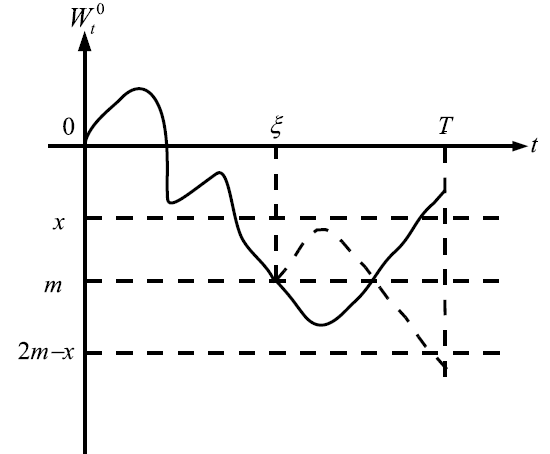
\includegraphics[scale=0.6]{figure5}
	\end{center}
	\label{reffig5}
	\caption{A graphical representation of the reflection principle of the Brownian motion $W_t$.}
\end{figure}

\newpage 
The dotted path after time $\xi$ is the mirror reflection of the Brownian path at the level m.
Suppose $W_T$ ends up at a value higher than x, then the reflected path at time $T$ has a value
lower than $2m − x$.

\subsubsection*{Quadratic Variation}

The quadratic varivation property of Bownian motion
\begin{itemize}
	\item $(dW_t)^2=dt$
	\item $dW_tdt=0$
	\item $(dt)^2=0$
	\item $(dW_t)^p=0, \hspace{0.3cm}p\geq3$
\end{itemize}\
Where ${W_t:t\geq 0}$ is a standard Brownian motion and $dW_t$ and $dt$ are the infinitesimal increment of $W_t$ and $t$, respectively. The significance of the above results constitutes the key ingredients in It\=o's formula to find the differential of a stochastic function and also in deriving the Black-Scholes equation to price option.
\subsubsection*{Geometric Brownian Motion}

The stock price cannot be negative (it is actually always positive, it just turns to zero when its company goes bankrupt). The stock price cannot be Browninan because the cycle of Brownian motion go to negative . But if we take logarithms of the stock price, it can be negative, and it can be imagined that the movement period  of the logarithms of the stock price  under the effect of random effects immediately on the market is similar to is the Browninan movement. Therefore, the following geometric Brownian motion concept is very important in describing the volatility of stock prices.\\[0.5cm]
GBM is the continuous time stochastic process $S_t$, which is defined by 
\begin{align*}
S_t=S_0e^{X_t} \label{x}
\end{align*}
where $X_t$ is Brownian motion with drift and $S(0)=S_0 \hspace{0.1cm} > \hspace{0.1cm} 0$ is the initial value. \\
The usual model for the time-evolution of an asset price $S_t$ is given by the GBM, represented by the following stochastic differential equation:
\begin{align*}
\dfrac{dS_t}{S_t}=\mu dt+\sigma dW_t
\end{align*}
The coefficients $\mu$ and $\sigma$, representing the drift and volatility of the asset, respectively, are both constant in this model.  \\[0.5cm]
Applying Taylor's theorem.\\[0.5cm]
Let $f(x)=\log S_t$
\begin{align*}
d(\log S_t)=df(x)=f^{\prime}(x)dx+\dfrac{1}{2}f^{\prime \prime}(x)dx^2=\dfrac{1}{x}dx+\dfrac{1}{2}(-\dfrac{1}{x^2})dx^2
\end{align*}
This leads to
\begin{align*}
d(logS_t)&=\dfrac{1}{S_t}dS_t+\dfrac{1}{2}\left(-\dfrac{1}{S_t^2}\right)dS_t^2\\
&=\dfrac{1}{S_t}(\mu S_tdt+\sigma S_tdW_t)-\dfrac{1}{2}\dfrac{(\mu S_tdt+\sigma S_tdW_t)^2}{S_t^2}\\
&=\mu dt+\sigma dW_t-\dfrac{1}{2}\dfrac{\sigma^2S_t^2dW_t^2}{S_t^2}\\
&=\mu dt+\sigma dW_t-\dfrac{\sigma^2dt}{2}\\
&=(\mu-\dfrac{\sigma^2}{2})dt+\sigma dW_t
\end{align*}
It is a standard Brownian motion with a drift term. Taking integral of  2 sides between the limits $0$ and $t$ we can write this as:
\begin{align*}
\int_{0}^{t}d(logS_u)&=\int_{0}^{t}\left(\mu -\dfrac{1}{2}\sigma^2 \right)u+\int_{0}^{t}\sigma W_u\\
logu|_0^t&=\left(\mu -\dfrac{1}{2}\sigma^2 \right)u\mid_0^t+\sigma W_u\mid_0^t\\
logS_t-logS_0&=\left(\mu -\dfrac{1}{2}\sigma^2 \right)(t-0)+\sigma(W_t-W_0)\\
logS_t-logS_0&=\left(\mu -\dfrac{1}{2}\sigma^2 \right)t+\sigma W_t\\
log\dfrac{S_t}{S_0}&=\left(\mu -\dfrac{1}{2}\sigma^2 \right)t+\sigma W_t
\end{align*}
Finally, taking the exponential of this equation gives:
\begin{align}
S_t=S_0e^{\left(\mu -\frac{1}{2}\sigma^2 \right)t+\sigma W_t}
\end{align} \label{eq2}

\section{Stochastic Differential Equations}

\textnormal A stochastic differential equation (SDE) is a differential equation in which one or more of
the terms has a random component. Within the context of mathematical finance, SDEs are
frequently used to model diverse phenomena such as stock prices, interest rates or volatilities
to name but a few. Typically, SDEs have continuous paths with both random and non-random
components and to drive the random component of the model they usually incorporate a Wiener
process.\\[0.5cm]
To begin with, a one-dimensional stochastic differential equation can be described as
\begin{align*}
dX_t=\mu(X_t,t)dt+\sigma(X_t,t)dW_t
\end{align*} 
where $W_t$ is a standard Wiener process, $\mu(X_t, t)$ is defined as the drift and $\sigma(X_t, t)$ the volatility.
Many financial models can be written in this form, such as the lognormal asset random walk,
common spot interest rate and stochastic volatility models.

\subsection{It\=o's lemma}
Ito's Lemma is a key component in the Ito Calculus, used to determine the derivative of a time-dependent function of a stochastic process.It can be heuristically derived by forming the Taylor series expansion of the function up to its second derivatives and retaining terms up to first order in the time increment and second order in the Wiener process increment. The lemma is widely employed in mathematical finance, and its best known application is in the derivation of the Black–Scholes equation for option values. Therefore, in order to derive It\=o's lemma we have to expand a Taylor series and applying the rules of stochastic calculus.

\subsubsection*{Taylor's Theorem}

Taylor's theorem in one real variable. \\
Let $k \geq 1$ be an integer and let the function $f : \mathbb{R} \to \mathbb{R}$ be $k$ times differentiable at the point $x_0 \in \mathbb{R}$ such that 
\begin{align*}
f(x)=f(x_0)+f^{\prime}(x_0)(x-x_0)+\dfrac{f^{\prime \prime}(x_0)}{2!}(x-x_0)^2+\dots+\dfrac{f^{(k)}(a)}{k!}(x-x_0)^k
\end{align*}
The partial derivatives through order 2 is given by
\begin{align*}
f(x)&=f(x_0)+f^{\prime}(x_0)(x-x_0)+\dfrac{f^{\prime \prime}(x_0)}{2!}(x-x_0)^2\\
f(x)-f(x_0)&=f^{\prime}(x_0)(x-x_0)+\dfrac{f^{\prime \prime}(x_0)}{2!}(x-x_0)^2\\
\Delta f(x)&=f^{\prime}(x_0)\Delta x+\dfrac{f^{\prime \prime}(x_0)}{2!}(\Delta x)^2
\end{align*}
When $\Delta x \rightarrow 0$ and $\Delta f(x) \rightarrow 0$.  This implies that
\begin{align*}
df(x)&=f^{\prime}(x)dx+\dfrac{1}{2}f^{\prime \prime}(x)dx^2
\end{align*}
Taylor's theorem in two real variable.  The partial derivatives of $f(x,t)$ through order 2 is 
\begin{align*}
df(x,t)=f^{\prime}_x(x,t)dx+f^{\prime}_t(x,t)dt+\dfrac{1}{2}f^{\prime \prime}_{x^2}(x,t)dx^2+\dfrac{1}{2}f^{\prime \prime}_{t^2}dt^2+f^{\prime \prime}_{xt}dxdt
\end{align*} 

\subsubsection*{Proof of It\=o's lemma}

Suppose that $f(X_t, t)$ is a continuous differential function of $t$ and $X_t$ follows 
\begin{align*}
dX_t=\mu_tdt+\sigma_tdW_t
\end{align*}
where $W_t$ is the Brownian motion. The variable $X_t$ has a drift rate of $\mu_t$ and has a variance rate of  $\sigma_t^2$. Applying Taylor's theorem in two variables $X_t$ and t we get
\begin{align*}
df(X_t,t)&=f^{\prime}_x(X_t,t)dX_t+f^{\prime}_t(X_t,t)dt+\dfrac{1}{2}f^{\prime \prime}_{x^2}(X_t,t)dX_t^2+\dfrac{1}{2}f^{\prime \prime}_{t^2}dt^2+f^{\prime \prime}_{xt}dX_tdt\\
\end{align*}
Based on the above quaratic variation property of Brownian motion we can obtain
\begin{align*}
df(X_t,t)&=f^{\prime}_x(X_t,t)dX_t+f^{\prime}_t(X_t,t)dt+\dfrac{1}{2}f^{\prime \prime}_{x^2}(X_t,t)dX_t^2+\dfrac{1}{2}f^{\prime \prime}_{t^2}0+f^{\prime \prime}_{xt}0\\
&=f^{\prime}_x(X_t,t)dX_t+f^{\prime}_t(X_t,t)dt+\dfrac{1}{2}f^{\prime \prime}_{x^2}(X_t,t)dX_t^2\\
&=f^\prime_x(X_t,t)(\mu_tdt+\sigma_tdW_t)+f^\prime_t(X_t,t)dt+\dfrac{1}{2}f^{\prime \prime}_{x^2}(X_t,t)(\mu_tdt+\sigma_tdW_t)^2\\
&=\left(f^\prime_t(X_t,t)+ \mu_tf^\prime_x(X_t,t)+\dfrac{\sigma_t^2}{2}f^{\prime \prime}_{x^2}(X_t,t)\right)dt+\sigma_t f^\prime_x(X_t,t)dW_t
\end{align*} 
Therefore, It\=o's lemma shows that a function $f$ of $X$ and $t$ follows the process 
\begin{align*}
df(X_t, t)=\left(\dfrac{\partial f}{\partial t}+\mu_t\dfrac{\partial f}{\partial x}+\dfrac{\sigma_t^2}{2}\dfrac{\partial^2 f}{\partial x^2}\right)dt+\sigma_t\dfrac{\partial f}{\partial x}dW_t
\end{align*}
\subsection{The Feynman-Kac formula}

Let $\{W_t: t \geq 0\}$ be a standard Wiener process on the probability space $(\Omega, \mathcal{F}, \mathbb{P})$ and let $\mathcal{F}_t$, $t \geq 0$ be the associated filtration. Let $X_t$ be the solution of the following SDE:
\begin{align*}
dX_t=\mu(X_t,t)dt+\sigma(X_t,t)dW_t
\end{align*} 
and define $r$ as a function of $t$. For $t\in [0,T]$ where $T \textgreater 0$ and if $V(X_t,t)$ satisfies the PDE
\begin{align}
\dfrac{\partial V}{\partial t}(X_t,t)+\dfrac{1}{2}\sigma(X_t,t)^2\dfrac{\partial^2V}{\partial X_t^2}(X_t,t)+\mu(X_t,t)\dfrac{\partial V}{\partial X_t}(X_t,t)-r(t)V(X_t,t)=0 \label{eq5.3.1}
\end{align} 
subject to the boundary condition $V(X_T,T)=\Psi (X_T)$, the under the filtration $\mathcal{F}_t$ the solution of the PDF is given by 
\begin{align*}
V(X_t,t)=\mathbb{E} \left[e^{-\int_{t}^{T}r(u)du}\Psi (X_T)\bigg|\mathcal{F}_t\right]
\end{align*}
By substituting $r(u)=r$, a constant. The time-t value $V(X_t; t)$ can be written as
\begin{align}
V(X_t; t)=e^{-r(T-t)}\mathbb{E}^\mathbb{Q}\left[\Psi (X_T)\bigg|\mathcal{F}_t\right]\label{eq5.3.2}
\end{align} 


